\section*{Appendix}
\subsection*{Introduction to MDP and the related terminologies}

A Markov Decision Process (MDP) consists of a finite set of states \(\mathcal{S}\),
a set of actions \(\mathcal{A}_s\), a real-valued reward function for each state-active pair
\(R(s,a)\) and the transition probabilities \(P(s' \mid s,a)\).

\subsubsection*{Policy}
A policy is a function that maps states to actions (or a distribution over actions).
In a deterministic world, it is given by \(\pi:\mathcal{S}_t \rightarrow \mathcal{A}_t\).
The aim of the agent is to learn the best policy mapping for the given problem.

\subsubsection*{Value Function}
For any policy \(\pi\) and state \(s\), \(V^\pi (s)\) is the value function, obeying policy \(\pi\).
It denotes the expected return from \(s\), given that the agent uses policy \(\pi\).
Return \(\mathcal{G}_t\), is the total reward obtained from the future steps.
When the number of stages (iterations), is finite, then the total reward makes sense.
However, in infinite-horizon cases, discounted return is used.
The value function is defined as follows:

\begin{equation}
    V^\pi (s)=E[r_{t+1}+\gamma r_{t+2}+ \gamma^2 r_{t+3} + \dots \mid s=s_t,\pi]
\end{equation}

where \(0 \leq \gamma  \leq 1\), is the discount factor.

\subsubsection*{Action Value Function}
Given a policy \(\pi\), current state \(s\) and an action chosen for the current state \(a\),
the action-value function, denoted by \(Q^\pi (s,a)\), is the expected infinite-horizon discounted return
for choosing action \(a\) in state \(s\). The action-value function is defined as follows:

\begin{equation}
    Q^\pi (s, a)=E[r_{t+1}+\gamma r_{t+2}+ \gamma^2 r_{t+3} + \dots \mid s=s_t, a=a_t, \pi]
\end{equation}

The optimal action-value, \(Q^*\) function maximizes the action-values for each state-action pair and
implicitly defines the optimal policy.

\subsection*{SMDP}

In hierarchical RL, the solutions to sub-problems are themselves considered as actions.
Different actions can take different time to execute.
This extension converts the problem from a MDP to a Semi Markov Decision process (SMDP).
A SMDP is defined like a MDP with an additional factor of \(\tau\), which is
a random variable denoting the time elapsed between decision stages.

The transition probabilities \(P(s', \tau \mid s,a)\) in a SMDP are
the joint probability of an agent transiting from state \(s\) to state \(s'\)  after \(\tau\)
time-steps by executing action \(a\).
The expected rewards \(R(s,a)\) denotes the reward accumulated by executing action
\(a\) in state \(s\) and waiting for \(\tau\) time-steps.

\subsection*{Optimality in Hierarchical RL}

In a flat reinforcement problem, optimality is achieved by solving the entire problem spawning through multiple
state spaces. However, this optimization is not straightforward with hierarchies.
Optimality can either be achieved granularly at each depth or else it can be achieved for the entire problem.
These differences bring about three different types of optimality in the HRL framework: Recursive, Hierarchical and Flat.

\subsubsection*{Recursive Optimality}
A policy is recursively optimal if the solutions to each of its sub-problems is optimal.
Such a solution respects the hierarchy but does not yield the globally optimal solution in all the cases.
Given the optimal policies to the sub-problems, a recursively optimal solution is simply the chain of these optimal sub-problems.

\iffalse
Consider a robotic agent in an environment with two rooms as given in Fig 1(a).
There are two passages between the two rooms. The task of the agent is to move from Room 1 to Room 2.
The actions available to the agent are moving in any of the four directions and the possible states
are the agent being in Room 1 in any of the three regions as defined by the two passages or the agent being in Room
2.  For simplicity, a 0 reward is kept aside for navigation and a reward of +1 for reaching the goal state.
The naive policy for the robot would be to opt the passage which is nearest to the robot and move out of the room.
However, assume that a goal is added to the scenario as shown in Fig 1 (b).
The task is now refined to navigate to the goal \(G\) in Room 2 from Room 1.
One of the policies which could be defined for this scenario is shown in Fig 1(c),
which is to move downwards in Room 2 and move in the direction of the passage which is nearer
both to the agent and the goal. Another valid policy, as given in Fig 1(d), would be to leave
Room 1 from the nearest passage and move downwards in Room 2. Note that in either cases,
the policy in Room 2 remains the same. The question is which one of these is optimal?
In the hierarchical set-up, both are optimal. The hierarchy in this case comes from the fact that
the entire problem is divided into two subtasks: exiting Room 1 through one of those passages and then
navigating to the goal. The former approach is hierarchically optimal whereas the later is recursively optimal.
This can be reasoned as the primary aim of the agent while solving the first subtask is to get out of Room 1
as efficiently as possible.
The agent overlooks the location of the goal in the second Room while considering recursive optimality.

\begin{figure}[ht] 
  \label{ Figure 1} 
  \begin{subfigure}[b]{0.5\linewidth}
    \centering
    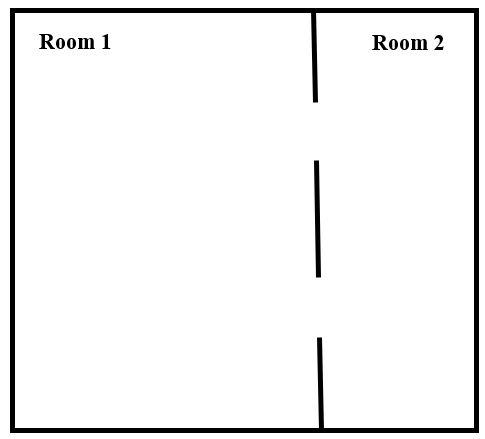
\includegraphics[width=.5\linewidth]{images/img1.JPG} 
    \caption{No goal} 
    \vspace{4ex}
  \end{subfigure}%%
  \begin{subfigure}[b]{0.5\linewidth}
    \centering
    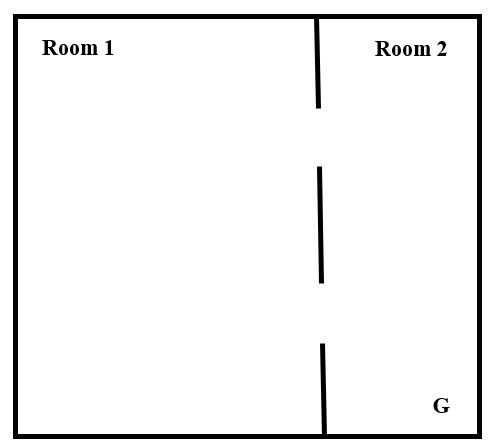
\includegraphics[width=.5\linewidth]{images/img2.JPG} 
    \caption{Goal in Room 2} 
    \vspace{4ex}
  \end{subfigure} 
  \begin{subfigure}[b]{0.5\linewidth}
    \centering
    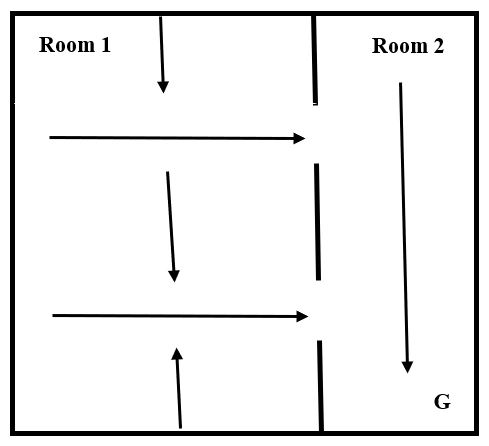
\includegraphics[width=.5\linewidth]{images/img3.JPG} 
    \caption{Hierarchically Optimal Solution} 
    \vspace{4ex}
  \end{subfigure}%% 
  \begin{subfigure}[b]{0.5\linewidth}
    \centering
    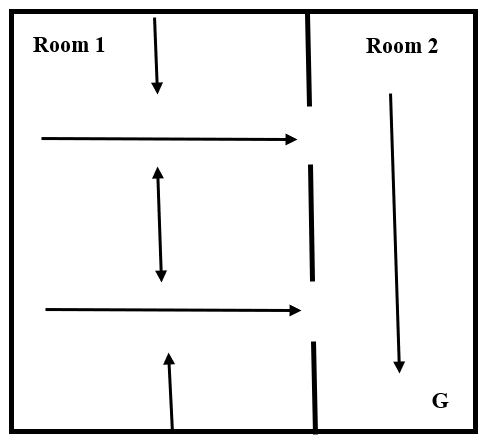
\includegraphics[width=.5\linewidth]{images/img4.JPG} 
    \caption{Recursively Optimal Solution} 
    \vspace{4ex}
  \end{subfigure} 
    \caption{Example to illustrate optimality}

\end{figure}
\fi

\subsubsection*{Hierarchical Optimality}

A policy is hierarchically optimal if it is the most optimal amongst all the policies that respect the hierarchy. Such a solution need not be optimal on each of its subproblems. In other words, in hierarchical optimality the presence of hierarchy is respected and is strictly adhered to. On the other hand, a recursive optimality keeps in mind the hierarchy but alters it to prioritize the subtasks first. As the overall hierarchy is put forth first, a solution with hierarchical optimality is always lesser than that of recursive optimality. Despite the con, recursive optimality gives the payoff of modularity. 


\subsubsection*{Flat Optimality}

Unlike the other two optimalitys, a flat solution does not respect hierarchy. It simply yields us the solution which is globally the most optimal. 
